
% Default to the notebook output style

    


% Inherit from the specified cell style.




    
\documentclass[11pt]{article}

    
    
    \usepackage[T1]{fontenc}
    % Nicer default font (+ math font) than Computer Modern for most use cases
    \usepackage{mathpazo}

    % Basic figure setup, for now with no caption control since it's done
    % automatically by Pandoc (which extracts ![](path) syntax from Markdown).
    \usepackage{graphicx}
    % We will generate all images so they have a width \maxwidth. This means
    % that they will get their normal width if they fit onto the page, but
    % are scaled down if they would overflow the margins.
    \makeatletter
    \def\maxwidth{\ifdim\Gin@nat@width>\linewidth\linewidth
    \else\Gin@nat@width\fi}
    \makeatother
    \let\Oldincludegraphics\includegraphics
    % Set max figure width to be 80% of text width, for now hardcoded.
    \renewcommand{\includegraphics}[1]{\Oldincludegraphics[width=.8\maxwidth]{#1}}
    % Ensure that by default, figures have no caption (until we provide a
    % proper Figure object with a Caption API and a way to capture that
    % in the conversion process - todo).
    \usepackage{caption}
    \DeclareCaptionLabelFormat{nolabel}{}
    \captionsetup{labelformat=nolabel}

    \usepackage{adjustbox} % Used to constrain images to a maximum size 
    \usepackage{xcolor} % Allow colors to be defined
    \usepackage{enumerate} % Needed for markdown enumerations to work
    \usepackage{geometry} % Used to adjust the document margins
    \usepackage{amsmath} % Equations
    \usepackage{amssymb} % Equations
    \usepackage{textcomp} % defines textquotesingle
    % Hack from http://tex.stackexchange.com/a/47451/13684:
    \AtBeginDocument{%
        \def\PYZsq{\textquotesingle}% Upright quotes in Pygmentized code
    }
    \usepackage{upquote} % Upright quotes for verbatim code
    \usepackage{eurosym} % defines \euro
    \usepackage[mathletters]{ucs} % Extended unicode (utf-8) support
    \usepackage[utf8x]{inputenc} % Allow utf-8 characters in the tex document
    \usepackage{fancyvrb} % verbatim replacement that allows latex
    \usepackage{grffile} % extends the file name processing of package graphics 
                         % to support a larger range 
    % The hyperref package gives us a pdf with properly built
    % internal navigation ('pdf bookmarks' for the table of contents,
    % internal cross-reference links, web links for URLs, etc.)
    \usepackage{hyperref}
    \usepackage{longtable} % longtable support required by pandoc >1.10
    \usepackage{booktabs}  % table support for pandoc > 1.12.2
    \usepackage[inline]{enumitem} % IRkernel/repr support (it uses the enumerate* environment)
    \usepackage[normalem]{ulem} % ulem is needed to support strikethroughs (\sout)
                                % normalem makes italics be italics, not underlines
    

    
    
    % Colors for the hyperref package
    \definecolor{urlcolor}{rgb}{0,.145,.698}
    \definecolor{linkcolor}{rgb}{.71,0.21,0.01}
    \definecolor{citecolor}{rgb}{.12,.54,.11}

    % ANSI colors
    \definecolor{ansi-black}{HTML}{3E424D}
    \definecolor{ansi-black-intense}{HTML}{282C36}
    \definecolor{ansi-red}{HTML}{E75C58}
    \definecolor{ansi-red-intense}{HTML}{B22B31}
    \definecolor{ansi-green}{HTML}{00A250}
    \definecolor{ansi-green-intense}{HTML}{007427}
    \definecolor{ansi-yellow}{HTML}{DDB62B}
    \definecolor{ansi-yellow-intense}{HTML}{B27D12}
    \definecolor{ansi-blue}{HTML}{208FFB}
    \definecolor{ansi-blue-intense}{HTML}{0065CA}
    \definecolor{ansi-magenta}{HTML}{D160C4}
    \definecolor{ansi-magenta-intense}{HTML}{A03196}
    \definecolor{ansi-cyan}{HTML}{60C6C8}
    \definecolor{ansi-cyan-intense}{HTML}{258F8F}
    \definecolor{ansi-white}{HTML}{C5C1B4}
    \definecolor{ansi-white-intense}{HTML}{A1A6B2}

    % commands and environments needed by pandoc snippets
    % extracted from the output of `pandoc -s`
    \providecommand{\tightlist}{%
      \setlength{\itemsep}{0pt}\setlength{\parskip}{0pt}}
    \DefineVerbatimEnvironment{Highlighting}{Verbatim}{commandchars=\\\{\}}
    % Add ',fontsize=\small' for more characters per line
    \newenvironment{Shaded}{}{}
    \newcommand{\KeywordTok}[1]{\textcolor[rgb]{0.00,0.44,0.13}{\textbf{{#1}}}}
    \newcommand{\DataTypeTok}[1]{\textcolor[rgb]{0.56,0.13,0.00}{{#1}}}
    \newcommand{\DecValTok}[1]{\textcolor[rgb]{0.25,0.63,0.44}{{#1}}}
    \newcommand{\BaseNTok}[1]{\textcolor[rgb]{0.25,0.63,0.44}{{#1}}}
    \newcommand{\FloatTok}[1]{\textcolor[rgb]{0.25,0.63,0.44}{{#1}}}
    \newcommand{\CharTok}[1]{\textcolor[rgb]{0.25,0.44,0.63}{{#1}}}
    \newcommand{\StringTok}[1]{\textcolor[rgb]{0.25,0.44,0.63}{{#1}}}
    \newcommand{\CommentTok}[1]{\textcolor[rgb]{0.38,0.63,0.69}{\textit{{#1}}}}
    \newcommand{\OtherTok}[1]{\textcolor[rgb]{0.00,0.44,0.13}{{#1}}}
    \newcommand{\AlertTok}[1]{\textcolor[rgb]{1.00,0.00,0.00}{\textbf{{#1}}}}
    \newcommand{\FunctionTok}[1]{\textcolor[rgb]{0.02,0.16,0.49}{{#1}}}
    \newcommand{\RegionMarkerTok}[1]{{#1}}
    \newcommand{\ErrorTok}[1]{\textcolor[rgb]{1.00,0.00,0.00}{\textbf{{#1}}}}
    \newcommand{\NormalTok}[1]{{#1}}
    
    % Additional commands for more recent versions of Pandoc
    \newcommand{\ConstantTok}[1]{\textcolor[rgb]{0.53,0.00,0.00}{{#1}}}
    \newcommand{\SpecialCharTok}[1]{\textcolor[rgb]{0.25,0.44,0.63}{{#1}}}
    \newcommand{\VerbatimStringTok}[1]{\textcolor[rgb]{0.25,0.44,0.63}{{#1}}}
    \newcommand{\SpecialStringTok}[1]{\textcolor[rgb]{0.73,0.40,0.53}{{#1}}}
    \newcommand{\ImportTok}[1]{{#1}}
    \newcommand{\DocumentationTok}[1]{\textcolor[rgb]{0.73,0.13,0.13}{\textit{{#1}}}}
    \newcommand{\AnnotationTok}[1]{\textcolor[rgb]{0.38,0.63,0.69}{\textbf{\textit{{#1}}}}}
    \newcommand{\CommentVarTok}[1]{\textcolor[rgb]{0.38,0.63,0.69}{\textbf{\textit{{#1}}}}}
    \newcommand{\VariableTok}[1]{\textcolor[rgb]{0.10,0.09,0.49}{{#1}}}
    \newcommand{\ControlFlowTok}[1]{\textcolor[rgb]{0.00,0.44,0.13}{\textbf{{#1}}}}
    \newcommand{\OperatorTok}[1]{\textcolor[rgb]{0.40,0.40,0.40}{{#1}}}
    \newcommand{\BuiltInTok}[1]{{#1}}
    \newcommand{\ExtensionTok}[1]{{#1}}
    \newcommand{\PreprocessorTok}[1]{\textcolor[rgb]{0.74,0.48,0.00}{{#1}}}
    \newcommand{\AttributeTok}[1]{\textcolor[rgb]{0.49,0.56,0.16}{{#1}}}
    \newcommand{\InformationTok}[1]{\textcolor[rgb]{0.38,0.63,0.69}{\textbf{\textit{{#1}}}}}
    \newcommand{\WarningTok}[1]{\textcolor[rgb]{0.38,0.63,0.69}{\textbf{\textit{{#1}}}}}
    
    
    % Define a nice break command that doesn't care if a line doesn't already
    % exist.
    \def\br{\hspace*{\fill} \\* }
    % Math Jax compatability definitions
    \def\gt{>}
    \def\lt{<}
    % Document parameters
    \title{Computing System}
    
    
    

    % Pygments definitions
    
\makeatletter
\def\PY@reset{\let\PY@it=\relax \let\PY@bf=\relax%
    \let\PY@ul=\relax \let\PY@tc=\relax%
    \let\PY@bc=\relax \let\PY@ff=\relax}
\def\PY@tok#1{\csname PY@tok@#1\endcsname}
\def\PY@toks#1+{\ifx\relax#1\empty\else%
    \PY@tok{#1}\expandafter\PY@toks\fi}
\def\PY@do#1{\PY@bc{\PY@tc{\PY@ul{%
    \PY@it{\PY@bf{\PY@ff{#1}}}}}}}
\def\PY#1#2{\PY@reset\PY@toks#1+\relax+\PY@do{#2}}

\expandafter\def\csname PY@tok@w\endcsname{\def\PY@tc##1{\textcolor[rgb]{0.73,0.73,0.73}{##1}}}
\expandafter\def\csname PY@tok@c\endcsname{\let\PY@it=\textit\def\PY@tc##1{\textcolor[rgb]{0.25,0.50,0.50}{##1}}}
\expandafter\def\csname PY@tok@cp\endcsname{\def\PY@tc##1{\textcolor[rgb]{0.74,0.48,0.00}{##1}}}
\expandafter\def\csname PY@tok@k\endcsname{\let\PY@bf=\textbf\def\PY@tc##1{\textcolor[rgb]{0.00,0.50,0.00}{##1}}}
\expandafter\def\csname PY@tok@kp\endcsname{\def\PY@tc##1{\textcolor[rgb]{0.00,0.50,0.00}{##1}}}
\expandafter\def\csname PY@tok@kt\endcsname{\def\PY@tc##1{\textcolor[rgb]{0.69,0.00,0.25}{##1}}}
\expandafter\def\csname PY@tok@o\endcsname{\def\PY@tc##1{\textcolor[rgb]{0.40,0.40,0.40}{##1}}}
\expandafter\def\csname PY@tok@ow\endcsname{\let\PY@bf=\textbf\def\PY@tc##1{\textcolor[rgb]{0.67,0.13,1.00}{##1}}}
\expandafter\def\csname PY@tok@nb\endcsname{\def\PY@tc##1{\textcolor[rgb]{0.00,0.50,0.00}{##1}}}
\expandafter\def\csname PY@tok@nf\endcsname{\def\PY@tc##1{\textcolor[rgb]{0.00,0.00,1.00}{##1}}}
\expandafter\def\csname PY@tok@nc\endcsname{\let\PY@bf=\textbf\def\PY@tc##1{\textcolor[rgb]{0.00,0.00,1.00}{##1}}}
\expandafter\def\csname PY@tok@nn\endcsname{\let\PY@bf=\textbf\def\PY@tc##1{\textcolor[rgb]{0.00,0.00,1.00}{##1}}}
\expandafter\def\csname PY@tok@ne\endcsname{\let\PY@bf=\textbf\def\PY@tc##1{\textcolor[rgb]{0.82,0.25,0.23}{##1}}}
\expandafter\def\csname PY@tok@nv\endcsname{\def\PY@tc##1{\textcolor[rgb]{0.10,0.09,0.49}{##1}}}
\expandafter\def\csname PY@tok@no\endcsname{\def\PY@tc##1{\textcolor[rgb]{0.53,0.00,0.00}{##1}}}
\expandafter\def\csname PY@tok@nl\endcsname{\def\PY@tc##1{\textcolor[rgb]{0.63,0.63,0.00}{##1}}}
\expandafter\def\csname PY@tok@ni\endcsname{\let\PY@bf=\textbf\def\PY@tc##1{\textcolor[rgb]{0.60,0.60,0.60}{##1}}}
\expandafter\def\csname PY@tok@na\endcsname{\def\PY@tc##1{\textcolor[rgb]{0.49,0.56,0.16}{##1}}}
\expandafter\def\csname PY@tok@nt\endcsname{\let\PY@bf=\textbf\def\PY@tc##1{\textcolor[rgb]{0.00,0.50,0.00}{##1}}}
\expandafter\def\csname PY@tok@nd\endcsname{\def\PY@tc##1{\textcolor[rgb]{0.67,0.13,1.00}{##1}}}
\expandafter\def\csname PY@tok@s\endcsname{\def\PY@tc##1{\textcolor[rgb]{0.73,0.13,0.13}{##1}}}
\expandafter\def\csname PY@tok@sd\endcsname{\let\PY@it=\textit\def\PY@tc##1{\textcolor[rgb]{0.73,0.13,0.13}{##1}}}
\expandafter\def\csname PY@tok@si\endcsname{\let\PY@bf=\textbf\def\PY@tc##1{\textcolor[rgb]{0.73,0.40,0.53}{##1}}}
\expandafter\def\csname PY@tok@se\endcsname{\let\PY@bf=\textbf\def\PY@tc##1{\textcolor[rgb]{0.73,0.40,0.13}{##1}}}
\expandafter\def\csname PY@tok@sr\endcsname{\def\PY@tc##1{\textcolor[rgb]{0.73,0.40,0.53}{##1}}}
\expandafter\def\csname PY@tok@ss\endcsname{\def\PY@tc##1{\textcolor[rgb]{0.10,0.09,0.49}{##1}}}
\expandafter\def\csname PY@tok@sx\endcsname{\def\PY@tc##1{\textcolor[rgb]{0.00,0.50,0.00}{##1}}}
\expandafter\def\csname PY@tok@m\endcsname{\def\PY@tc##1{\textcolor[rgb]{0.40,0.40,0.40}{##1}}}
\expandafter\def\csname PY@tok@gh\endcsname{\let\PY@bf=\textbf\def\PY@tc##1{\textcolor[rgb]{0.00,0.00,0.50}{##1}}}
\expandafter\def\csname PY@tok@gu\endcsname{\let\PY@bf=\textbf\def\PY@tc##1{\textcolor[rgb]{0.50,0.00,0.50}{##1}}}
\expandafter\def\csname PY@tok@gd\endcsname{\def\PY@tc##1{\textcolor[rgb]{0.63,0.00,0.00}{##1}}}
\expandafter\def\csname PY@tok@gi\endcsname{\def\PY@tc##1{\textcolor[rgb]{0.00,0.63,0.00}{##1}}}
\expandafter\def\csname PY@tok@gr\endcsname{\def\PY@tc##1{\textcolor[rgb]{1.00,0.00,0.00}{##1}}}
\expandafter\def\csname PY@tok@ge\endcsname{\let\PY@it=\textit}
\expandafter\def\csname PY@tok@gs\endcsname{\let\PY@bf=\textbf}
\expandafter\def\csname PY@tok@gp\endcsname{\let\PY@bf=\textbf\def\PY@tc##1{\textcolor[rgb]{0.00,0.00,0.50}{##1}}}
\expandafter\def\csname PY@tok@go\endcsname{\def\PY@tc##1{\textcolor[rgb]{0.53,0.53,0.53}{##1}}}
\expandafter\def\csname PY@tok@gt\endcsname{\def\PY@tc##1{\textcolor[rgb]{0.00,0.27,0.87}{##1}}}
\expandafter\def\csname PY@tok@err\endcsname{\def\PY@bc##1{\setlength{\fboxsep}{0pt}\fcolorbox[rgb]{1.00,0.00,0.00}{1,1,1}{\strut ##1}}}
\expandafter\def\csname PY@tok@kc\endcsname{\let\PY@bf=\textbf\def\PY@tc##1{\textcolor[rgb]{0.00,0.50,0.00}{##1}}}
\expandafter\def\csname PY@tok@kd\endcsname{\let\PY@bf=\textbf\def\PY@tc##1{\textcolor[rgb]{0.00,0.50,0.00}{##1}}}
\expandafter\def\csname PY@tok@kn\endcsname{\let\PY@bf=\textbf\def\PY@tc##1{\textcolor[rgb]{0.00,0.50,0.00}{##1}}}
\expandafter\def\csname PY@tok@kr\endcsname{\let\PY@bf=\textbf\def\PY@tc##1{\textcolor[rgb]{0.00,0.50,0.00}{##1}}}
\expandafter\def\csname PY@tok@bp\endcsname{\def\PY@tc##1{\textcolor[rgb]{0.00,0.50,0.00}{##1}}}
\expandafter\def\csname PY@tok@fm\endcsname{\def\PY@tc##1{\textcolor[rgb]{0.00,0.00,1.00}{##1}}}
\expandafter\def\csname PY@tok@vc\endcsname{\def\PY@tc##1{\textcolor[rgb]{0.10,0.09,0.49}{##1}}}
\expandafter\def\csname PY@tok@vg\endcsname{\def\PY@tc##1{\textcolor[rgb]{0.10,0.09,0.49}{##1}}}
\expandafter\def\csname PY@tok@vi\endcsname{\def\PY@tc##1{\textcolor[rgb]{0.10,0.09,0.49}{##1}}}
\expandafter\def\csname PY@tok@vm\endcsname{\def\PY@tc##1{\textcolor[rgb]{0.10,0.09,0.49}{##1}}}
\expandafter\def\csname PY@tok@sa\endcsname{\def\PY@tc##1{\textcolor[rgb]{0.73,0.13,0.13}{##1}}}
\expandafter\def\csname PY@tok@sb\endcsname{\def\PY@tc##1{\textcolor[rgb]{0.73,0.13,0.13}{##1}}}
\expandafter\def\csname PY@tok@sc\endcsname{\def\PY@tc##1{\textcolor[rgb]{0.73,0.13,0.13}{##1}}}
\expandafter\def\csname PY@tok@dl\endcsname{\def\PY@tc##1{\textcolor[rgb]{0.73,0.13,0.13}{##1}}}
\expandafter\def\csname PY@tok@s2\endcsname{\def\PY@tc##1{\textcolor[rgb]{0.73,0.13,0.13}{##1}}}
\expandafter\def\csname PY@tok@sh\endcsname{\def\PY@tc##1{\textcolor[rgb]{0.73,0.13,0.13}{##1}}}
\expandafter\def\csname PY@tok@s1\endcsname{\def\PY@tc##1{\textcolor[rgb]{0.73,0.13,0.13}{##1}}}
\expandafter\def\csname PY@tok@mb\endcsname{\def\PY@tc##1{\textcolor[rgb]{0.40,0.40,0.40}{##1}}}
\expandafter\def\csname PY@tok@mf\endcsname{\def\PY@tc##1{\textcolor[rgb]{0.40,0.40,0.40}{##1}}}
\expandafter\def\csname PY@tok@mh\endcsname{\def\PY@tc##1{\textcolor[rgb]{0.40,0.40,0.40}{##1}}}
\expandafter\def\csname PY@tok@mi\endcsname{\def\PY@tc##1{\textcolor[rgb]{0.40,0.40,0.40}{##1}}}
\expandafter\def\csname PY@tok@il\endcsname{\def\PY@tc##1{\textcolor[rgb]{0.40,0.40,0.40}{##1}}}
\expandafter\def\csname PY@tok@mo\endcsname{\def\PY@tc##1{\textcolor[rgb]{0.40,0.40,0.40}{##1}}}
\expandafter\def\csname PY@tok@ch\endcsname{\let\PY@it=\textit\def\PY@tc##1{\textcolor[rgb]{0.25,0.50,0.50}{##1}}}
\expandafter\def\csname PY@tok@cm\endcsname{\let\PY@it=\textit\def\PY@tc##1{\textcolor[rgb]{0.25,0.50,0.50}{##1}}}
\expandafter\def\csname PY@tok@cpf\endcsname{\let\PY@it=\textit\def\PY@tc##1{\textcolor[rgb]{0.25,0.50,0.50}{##1}}}
\expandafter\def\csname PY@tok@c1\endcsname{\let\PY@it=\textit\def\PY@tc##1{\textcolor[rgb]{0.25,0.50,0.50}{##1}}}
\expandafter\def\csname PY@tok@cs\endcsname{\let\PY@it=\textit\def\PY@tc##1{\textcolor[rgb]{0.25,0.50,0.50}{##1}}}

\def\PYZbs{\char`\\}
\def\PYZus{\char`\_}
\def\PYZob{\char`\{}
\def\PYZcb{\char`\}}
\def\PYZca{\char`\^}
\def\PYZam{\char`\&}
\def\PYZlt{\char`\<}
\def\PYZgt{\char`\>}
\def\PYZsh{\char`\#}
\def\PYZpc{\char`\%}
\def\PYZdl{\char`\$}
\def\PYZhy{\char`\-}
\def\PYZsq{\char`\'}
\def\PYZdq{\char`\"}
\def\PYZti{\char`\~}
% for compatibility with earlier versions
\def\PYZat{@}
\def\PYZlb{[}
\def\PYZrb{]}
\makeatother


    % Exact colors from NB
    \definecolor{incolor}{rgb}{0.0, 0.0, 0.5}
    \definecolor{outcolor}{rgb}{0.545, 0.0, 0.0}



    
    % Prevent overflowing lines due to hard-to-break entities
    \sloppy 
    % Setup hyperref package
    \hypersetup{
      breaklinks=true,  % so long urls are correctly broken across lines
      colorlinks=true,
      urlcolor=urlcolor,
      linkcolor=linkcolor,
      citecolor=citecolor,
      }
    % Slightly bigger margins than the latex defaults
    
    \geometry{verbose,tmargin=1in,bmargin=1in,lmargin=1in,rmargin=1in}
    
    

    \begin{document}
    
    
    \maketitle
    
    

    
    \hypertarget{introduction}{%
\section{Introduction}\label{introduction}}

    The goal of this document is to construct a computer from logical gates.
The basic logical gates that are used to construct the computer are:
\texttt{And}, \texttt{Or}, and \texttt{Not}. The major outline of this
document is followed from the book \emph{The Elements of Computing
Systems, Noam Nisan and Shimon Shocken (2008)}.

The book is followed from Boolean Logic (chapter 1) to Assembler
(chapter 6). The construction of the Virtual Machine, and eventually an
Operating System, is left out of scope. The main reason for this, is
because Python does not allow an easy `screen' interface. The entire
emulator will be written as a \texttt{REPL} application, which allows
the user excessive control of the entire emulator. The cost of this,
however, is that everything is done at a very low level.

The goal is to create a computer that can run Assembly code, and that we
have an assembler. I haven't followed the Assembly implementation in the
book, instead, I used it as a baseline, and transformed it into my own
preferences.

    \hypertarget{boolean-logic}{%
\section{Boolean logic}\label{boolean-logic}}

    Every Boolean function, no matter how complex, can be expressed using
three Boolean operators only: \texttt{And}, \texttt{Or}, and
\texttt{Not}.

    \hypertarget{gate-logic}{%
\subsection{Gate logic}\label{gate-logic}}

    A \emph{gate} is a physical device that implements a Boolean function.
If a Boolean function \(f\) operates on \(n\) variables and returns
\(m\) binary results, the gate that implements \(f\) will have
\emph{\(n\) input pins and \(m\) output pins}. Today, most gates are
implemented as transistors etched in silicon, packaged as \emph{chips}.

There are the following three \emph{primitive gates}, which will be used
to create all the other components. The gates are: \texttt{And},
\texttt{Or}, and \texttt{Not}. The following symbols are used to
indicate each gate:

\begin{figure}
\centering
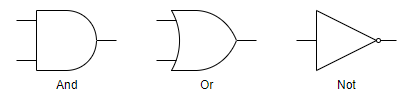
\includegraphics{gates1.PNG}
\caption{Primitive gates}
\end{figure}

We can define their Boolean functions mathematically as:

\begin{enumerate}
\def\labelenumi{\arabic{enumi}.}
\tightlist
\item
  \(\text{And}(a,b)=a\land b\)
\item
  \(\text{Or}(a,b)=a\lor b\)
\item
  \(\text{Not}(a)=\lnot a\)
\end{enumerate}

For ease of writing, we will also adopt the convention to write a \(1\)
when the value is \texttt{True}, and \(0\) if the value is
\texttt{False}.

    \hypertarget{primitive-gates}{%
\subsection{Primitive gates}\label{primitive-gates}}

    We will now implement the primitive logic gates in Python. The input
variables can be either a Boolean value, or a function. The input will
be called by the \texttt{boolf(x)} function, which returns a Boolean
value, or executes the function. Allowing functions gives us the option
to easily chain multiple gates together with references.

    \begin{Verbatim}[commandchars=\\\{\}]
{\color{incolor}In [{\color{incolor}21}]:} \PY{k}{def} \PY{n+nf}{boolf}\PY{p}{(}\PY{n}{x}\PY{p}{)}\PY{p}{:}
             \PY{k}{if} \PY{n}{callable}\PY{p}{(}\PY{n}{x}\PY{p}{)}\PY{p}{:} \PY{k}{return} \PY{n}{x}\PY{p}{(}\PY{p}{)}
             \PY{k}{if} \PY{n+nb}{type}\PY{p}{(}\PY{n}{x}\PY{p}{)} \PY{o+ow}{is} \PY{n+nb}{bool}\PY{p}{:} \PY{k}{return} \PY{n}{x}
             \PY{k}{raise} \PY{n+ne}{ValueError}\PY{p}{(}\PY{l+s+s1}{\PYZsq{}}\PY{l+s+s1}{Unsupported type }\PY{l+s+si}{\PYZob{}\PYZcb{}}\PY{l+s+s1}{ for boolf()}\PY{l+s+s1}{\PYZsq{}}\PY{o}{.}\PY{n}{format}\PY{p}{(}\PY{n+nb}{type}\PY{p}{(}\PY{n}{x}\PY{p}{)}\PY{p}{)}\PY{p}{)}
\end{Verbatim}


    \begin{Verbatim}[commandchars=\\\{\}]
{\color{incolor}In [{\color{incolor}17}]:} \PY{k}{class} \PY{n+nc}{And}\PY{p}{(}\PY{p}{)}\PY{p}{:}
             \PY{k}{def} \PY{n+nf}{\PYZus{}\PYZus{}init\PYZus{}\PYZus{}}\PY{p}{(}\PY{n+nb+bp}{self}\PY{p}{,} \PY{n}{a}\PY{p}{,} \PY{n}{b}\PY{p}{)}\PY{p}{:} \PY{n+nb+bp}{self}\PY{o}{.}\PY{n}{a} \PY{o}{=} \PY{n}{a}\PY{p}{;} \PY{n+nb+bp}{self}\PY{o}{.}\PY{n}{b} \PY{o}{=} \PY{n}{b}
             \PY{k}{def} \PY{n+nf}{out}\PY{p}{(}\PY{n+nb+bp}{self}\PY{p}{)}\PY{p}{:} \PY{k}{return} \PY{n}{boolf}\PY{p}{(}\PY{n+nb+bp}{self}\PY{o}{.}\PY{n}{a}\PY{p}{)} \PY{o+ow}{and} \PY{n}{boolf}\PY{p}{(}\PY{n+nb+bp}{self}\PY{o}{.}\PY{n}{b}\PY{p}{)}
             \PY{k}{def} \PY{n+nf}{\PYZus{}\PYZus{}repr\PYZus{}\PYZus{}}\PY{p}{(}\PY{n+nb+bp}{self}\PY{p}{)}\PY{p}{:} \PY{k}{return} \PY{l+s+s1}{\PYZsq{}}\PY{l+s+si}{\PYZob{}\PYZcb{}}\PY{l+s+s1}{\PYZsq{}}\PY{o}{.}\PY{n}{format}\PY{p}{(}\PY{n+nb+bp}{self}\PY{o}{.}\PY{n}{out}\PY{p}{(}\PY{p}{)}\PY{p}{)}
         
         \PY{k}{class} \PY{n+nc}{Or}\PY{p}{(}\PY{p}{)}\PY{p}{:}
             \PY{k}{def} \PY{n+nf}{\PYZus{}\PYZus{}init\PYZus{}\PYZus{}}\PY{p}{(}\PY{n+nb+bp}{self}\PY{p}{,} \PY{n}{a}\PY{p}{,} \PY{n}{b}\PY{p}{)}\PY{p}{:} \PY{n+nb+bp}{self}\PY{o}{.}\PY{n}{a} \PY{o}{=} \PY{n}{a}\PY{p}{;} \PY{n+nb+bp}{self}\PY{o}{.}\PY{n}{b} \PY{o}{=} \PY{n}{b}
             \PY{k}{def} \PY{n+nf}{out}\PY{p}{(}\PY{n+nb+bp}{self}\PY{p}{)}\PY{p}{:} \PY{k}{return} \PY{n}{boolf}\PY{p}{(}\PY{n+nb+bp}{self}\PY{o}{.}\PY{n}{a}\PY{p}{)} \PY{o+ow}{or} \PY{n}{boolf}\PY{p}{(}\PY{n+nb+bp}{self}\PY{o}{.}\PY{n}{b}\PY{p}{)}
             \PY{k}{def} \PY{n+nf}{\PYZus{}\PYZus{}repr\PYZus{}\PYZus{}}\PY{p}{(}\PY{n+nb+bp}{self}\PY{p}{)}\PY{p}{:} \PY{k}{return} \PY{l+s+s1}{\PYZsq{}}\PY{l+s+si}{\PYZob{}\PYZcb{}}\PY{l+s+s1}{\PYZsq{}}\PY{o}{.}\PY{n}{format}\PY{p}{(}\PY{n+nb+bp}{self}\PY{o}{.}\PY{n}{out}\PY{p}{(}\PY{p}{)}\PY{p}{)}
             
         \PY{k}{class} \PY{n+nc}{Not}\PY{p}{(}\PY{p}{)}\PY{p}{:}
             \PY{k}{def} \PY{n+nf}{\PYZus{}\PYZus{}init\PYZus{}\PYZus{}}\PY{p}{(}\PY{n+nb+bp}{self}\PY{p}{,} \PY{n}{a}\PY{p}{)}\PY{p}{:} \PY{n+nb+bp}{self}\PY{o}{.}\PY{n}{a} \PY{o}{=} \PY{n}{a}
             \PY{k}{def} \PY{n+nf}{out}\PY{p}{(}\PY{n+nb+bp}{self}\PY{p}{)}\PY{p}{:} \PY{k}{return} \PY{o+ow}{not} \PY{n}{boolf}\PY{p}{(}\PY{n+nb+bp}{self}\PY{o}{.}\PY{n}{a}\PY{p}{)}
             \PY{k}{def} \PY{n+nf}{\PYZus{}\PYZus{}repr\PYZus{}\PYZus{}}\PY{p}{(}\PY{n+nb+bp}{self}\PY{p}{)}\PY{p}{:} \PY{k}{return} \PY{l+s+s1}{\PYZsq{}}\PY{l+s+si}{\PYZob{}\PYZcb{}}\PY{l+s+s1}{\PYZsq{}}\PY{o}{.}\PY{n}{format}\PY{p}{(}\PY{n+nb+bp}{self}\PY{o}{.}\PY{n}{out}\PY{p}{(}\PY{p}{)}\PY{p}{)}
\end{Verbatim}


    To test a simple scenario, let
\(G(a,b,c) = \text{Not}(\text{Or}(a, \text{And}(b, c)))\). Because this
is a composite gate, we are only using primitive gates. If
\((a,b,c)=(0,1,1)\), the resulting output should be \(0\).

    \begin{Verbatim}[commandchars=\\\{\}]
{\color{incolor}In [{\color{incolor}49}]:} \PY{n}{a}\PY{o}{=}\PY{k+kc}{False}\PY{p}{;}\PY{n}{b}\PY{o}{=}\PY{n}{c}\PY{o}{=}\PY{k+kc}{True}
         \PY{n}{G} \PY{o}{=} \PY{n}{Not}\PY{p}{(}\PY{n}{Or}\PY{p}{(}\PY{k}{lambda}\PY{p}{:} \PY{n}{a}\PY{p}{,} \PY{n}{And}\PY{p}{(}\PY{k}{lambda}\PY{p}{:} \PY{n}{b}\PY{p}{,} \PY{k}{lambda}\PY{p}{:} \PY{n}{c}\PY{p}{)}\PY{o}{.}\PY{n}{out}\PY{p}{)}\PY{o}{.}\PY{n}{out}\PY{p}{)}
         \PY{n+nb}{print}\PY{p}{(}\PY{n}{G}\PY{p}{)}
         
         \PY{n}{b}\PY{o}{=}\PY{k+kc}{False}
         \PY{n+nb}{print}\PY{p}{(}\PY{n}{G}\PY{p}{)}
\end{Verbatim}


    \begin{Verbatim}[commandchars=\\\{\}]
False
True

    \end{Verbatim}

    \textbf{Reference vs.~value types}

Notice that primitive Boolean values should be the result of a function.
If a Boolean value is the input for a gate, Python will reference to it
by value, which is something we do not want. Thus, we input a function
into the gate, and Python passes the function as a reference. Then we
use \texttt{boolf(x)} to either get the variable, or return the function
result. This allows us to change the input values, after the gate has
been constructed, and keep calling \texttt{.out()} on the last gate to
execute all the logic in the intermediate gates.

    \hypertarget{composite-gates}{%
\subsection{Composite gates}\label{composite-gates}}

    We start with primitive gates and design more complicated functionality
by interconnecting them, leading to the construction of \emph{composite
gates}.

    \hypertarget{three-way-and-gate}{%
\subsubsection{Three-way and gate}\label{three-way-and-gate}}

    The first gate we can construct from two and gates, is a three-way and
gate. It can be defined in the following way:
\(\text{And3W}(a,b,c)= \text{And}(\text{And}(a,b),c)\).

\begin{figure}
\centering
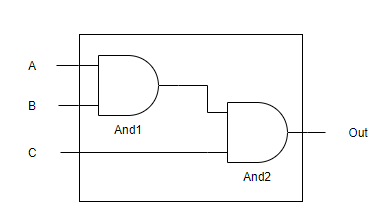
\includegraphics{gates2.PNG}
\caption{Three-way and gate diagram}
\end{figure}

    \begin{Verbatim}[commandchars=\\\{\}]
{\color{incolor}In [{\color{incolor}19}]:} \PY{k}{class} \PY{n+nc}{And3W}\PY{p}{(}\PY{p}{)}\PY{p}{:}
             \PY{k}{def} \PY{n+nf}{\PYZus{}\PYZus{}init\PYZus{}\PYZus{}}\PY{p}{(}\PY{n+nb+bp}{self}\PY{p}{,} \PY{n}{a}\PY{p}{,} \PY{n}{b}\PY{p}{,} \PY{n}{c}\PY{p}{)}\PY{p}{:} \PY{n+nb+bp}{self}\PY{o}{.}\PY{n}{a} \PY{o}{=} \PY{n}{a}\PY{p}{;} \PY{n+nb+bp}{self}\PY{o}{.}\PY{n}{b} \PY{o}{=} \PY{n}{b}\PY{p}{;} \PY{n+nb+bp}{self}\PY{o}{.}\PY{n}{c} \PY{o}{=} \PY{n}{c}
             \PY{k}{def} \PY{n+nf}{out}\PY{p}{(}\PY{n+nb+bp}{self}\PY{p}{)}\PY{p}{:} 
                 \PY{n}{and1} \PY{o}{=} \PY{n}{And}\PY{p}{(}\PY{n}{boolf}\PY{p}{(}\PY{n+nb+bp}{self}\PY{o}{.}\PY{n}{a}\PY{p}{)}\PY{p}{,} \PY{n}{boolf}\PY{p}{(}\PY{n+nb+bp}{self}\PY{o}{.}\PY{n}{b}\PY{p}{)}\PY{p}{)}
                 \PY{n}{and2} \PY{o}{=} \PY{n}{And}\PY{p}{(}\PY{n}{and1}\PY{o}{.}\PY{n}{out}\PY{p}{,} \PY{n}{boolf}\PY{p}{(}\PY{n+nb+bp}{self}\PY{o}{.}\PY{n}{c}\PY{p}{)}\PY{p}{)}
                 \PY{k}{return} \PY{n}{and2}\PY{o}{.}\PY{n}{out}\PY{p}{(}\PY{p}{)}
             \PY{k}{def} \PY{n+nf}{\PYZus{}\PYZus{}repr\PYZus{}\PYZus{}}\PY{p}{(}\PY{n+nb+bp}{self}\PY{p}{)}\PY{p}{:} \PY{k}{return} \PY{l+s+s1}{\PYZsq{}}\PY{l+s+si}{\PYZob{}\PYZcb{}}\PY{l+s+s1}{\PYZsq{}}\PY{o}{.}\PY{n}{format}\PY{p}{(}\PY{n+nb+bp}{self}\PY{o}{.}\PY{n}{out}\PY{p}{(}\PY{p}{)}\PY{p}{)}
\end{Verbatim}


    \begin{Verbatim}[commandchars=\\\{\}]
{\color{incolor}In [{\color{incolor}20}]:} \PY{n}{And3W}\PY{p}{(}\PY{k+kc}{True}\PY{p}{,} \PY{k+kc}{True}\PY{p}{,} \PY{k+kc}{True}\PY{p}{)}
\end{Verbatim}


\begin{Verbatim}[commandchars=\\\{\}]
{\color{outcolor}Out[{\color{outcolor}20}]:} True
\end{Verbatim}
            
    \hypertarget{xor-gate}{%
\subsubsection{Xor gate}\label{xor-gate}}

    Let us consider another logic design example -- that of a \texttt{Xor}
gate. The gate \(\text{Xor}(a,b)\) is \(1\) exactly when \(a=1\) and
\(b=0\), or \(a=0\) and \(b=1\). In the case where \(a=b\) the gate is
\(0\). It can be defined in the following way:
\(\text{Xor(a,b)}=\text{Or}(\text{And}(a,\text{Not}(b)), \text{And}(\text{Not}(a),b))\).
This definition leads to the logic design shown in the figure below:

    \begin{Verbatim}[commandchars=\\\{\}]
{\color{incolor}In [{\color{incolor}77}]:} \PY{k}{class} \PY{n+nc}{Xor}\PY{p}{(}\PY{p}{)}\PY{p}{:}
             \PY{k}{def} \PY{n+nf}{\PYZus{}\PYZus{}init\PYZus{}\PYZus{}}\PY{p}{(}\PY{n+nb+bp}{self}\PY{p}{,} \PY{n}{a}\PY{p}{,} \PY{n}{b}\PY{p}{)}\PY{p}{:} \PY{n+nb+bp}{self}\PY{o}{.}\PY{n}{a} \PY{o}{=} \PY{n}{a}\PY{p}{;} \PY{n+nb+bp}{self}\PY{o}{.}\PY{n}{b} \PY{o}{=} \PY{n}{b}
             \PY{k}{def} \PY{n+nf}{out}\PY{p}{(}\PY{n+nb+bp}{self}\PY{p}{)}\PY{p}{:} \PY{k}{return} \PY{n}{Or}\PY{p}{(}\PY{n}{And}\PY{p}{(}\PY{n}{boolf}\PY{p}{(}\PY{n+nb+bp}{self}\PY{o}{.}\PY{n}{a}\PY{p}{)}\PY{p}{,} \PY{n}{Not}\PY{p}{(}\PY{n}{boolf}\PY{p}{(}\PY{n+nb+bp}{self}\PY{o}{.}\PY{n}{b}\PY{p}{)}\PY{p}{)}\PY{o}{.}\PY{n}{out}\PY{p}{)}\PY{o}{.}\PY{n}{out}\PY{p}{,}\PYZbs{}
                                      \PY{n}{And}\PY{p}{(}\PY{n}{Not}\PY{p}{(}\PY{n}{boolf}\PY{p}{(}\PY{n+nb+bp}{self}\PY{o}{.}\PY{n}{a}\PY{p}{)}\PY{p}{)}\PY{o}{.}\PY{n}{out}\PY{p}{,} \PY{n}{boolf}\PY{p}{(}\PY{n+nb+bp}{self}\PY{o}{.}\PY{n}{b}\PY{p}{)}\PY{p}{)}\PY{o}{.}\PY{n}{out}\PYZbs{}
                                   \PY{p}{)}\PY{o}{.}\PY{n}{out}\PY{p}{(}\PY{p}{)}
             \PY{k}{def} \PY{n+nf}{\PYZus{}\PYZus{}repr\PYZus{}\PYZus{}}\PY{p}{(}\PY{n+nb+bp}{self}\PY{p}{)}\PY{p}{:} \PY{k}{return} \PY{l+s+s1}{\PYZsq{}}\PY{l+s+si}{\PYZob{}\PYZcb{}}\PY{l+s+s1}{\PYZsq{}}\PY{o}{.}\PY{n}{format}\PY{p}{(}\PY{n+nb+bp}{self}\PY{o}{.}\PY{n}{out}\PY{p}{(}\PY{p}{)}\PY{p}{)}
\end{Verbatim}


    \begin{Verbatim}[commandchars=\\\{\}]
{\color{incolor}In [{\color{incolor}86}]:} \PY{n}{Xor}\PY{p}{(}\PY{k+kc}{False}\PY{p}{,} \PY{k+kc}{True}\PY{p}{)}\PY{o}{.}\PY{n}{out}\PY{p}{(}\PY{p}{)} \PY{o+ow}{and} \PY{n}{Xor}\PY{p}{(}\PY{k+kc}{True}\PY{p}{,} \PY{k+kc}{False}\PY{p}{)}\PY{o}{.}\PY{n}{out}\PY{p}{(}\PY{p}{)} \PYZbs{}
             \PY{o+ow}{and} \PY{o+ow}{not} \PY{n}{Xor}\PY{p}{(}\PY{k+kc}{True}\PY{p}{,} \PY{k+kc}{True}\PY{p}{)}\PY{o}{.}\PY{n}{out}\PY{p}{(}\PY{p}{)} \PY{o+ow}{and} \PY{o+ow}{not} \PY{n}{Xor}\PY{p}{(}\PY{k+kc}{False}\PY{p}{,} \PY{k+kc}{False}\PY{p}{)}\PY{o}{.}\PY{n}{out}\PY{p}{(}\PY{p}{)}
\end{Verbatim}


\begin{Verbatim}[commandchars=\\\{\}]
{\color{outcolor}Out[{\color{outcolor}86}]:} True
\end{Verbatim}
            
    \hypertarget{basic-logic-gates}{%
\subsection{Basic Logic Gates}\label{basic-logic-gates}}

    \hypertarget{not}{%
\subsubsection{Not}\label{not}}

    \hypertarget{and}{%
\subsubsection{And}\label{and}}

    \hypertarget{or}{%
\subsubsection{Or}\label{or}}

    \hypertarget{xor}{%
\subsubsection{Xor}\label{xor}}

    \hypertarget{multiplexor}{%
\subsubsection{Multiplexor}\label{multiplexor}}

    \hypertarget{demultiplexor}{%
\subsubsection{Demultiplexor}\label{demultiplexor}}

    \hypertarget{multi-bit-versions-of-basic-gates}{%
\subsection{Multi-bit Versions of Basic
gates}\label{multi-bit-versions-of-basic-gates}}

    \hypertarget{not16}{%
\subsubsection{Not16}\label{not16}}

    \hypertarget{and16}{%
\subsubsection{And16}\label{and16}}

    \hypertarget{or16}{%
\subsubsection{Or16}\label{or16}}

    \hypertarget{mux16}{%
\subsubsection{Mux16}\label{mux16}}

    \hypertarget{multi-way-versions-of-basic-gates}{%
\subsection{Multi-Way Versions of Basic
Gates}\label{multi-way-versions-of-basic-gates}}

    \hypertarget{or8way}{%
\subsubsection{Or8Way}\label{or8way}}

    \hypertarget{multi-waymulti-bit-multiplexor}{%
\subsubsection{Multi-Way/Multi-Bit
Multiplexor}\label{multi-waymulti-bit-multiplexor}}

    \hypertarget{mux4way16}{%
\paragraph{Mux4Way16}\label{mux4way16}}

    \hypertarget{mux8way16}{%
\paragraph{Mux8Way16}\label{mux8way16}}

    \hypertarget{dmux4way}{%
\paragraph{DMux4Way}\label{dmux4way}}

    \hypertarget{dmux8way}{%
\paragraph{DMux8Way}\label{dmux8way}}

    \hypertarget{boolean-arithmetic}{%
\section{Boolean Arithmetic}\label{boolean-arithmetic}}

    \hypertarget{sequential-logic}{%
\section{Sequential Logic}\label{sequential-logic}}

    \hypertarget{machine-language}{%
\section{Machine Language}\label{machine-language}}

    \hypertarget{computer-architecture}{%
\section{Computer Architecture}\label{computer-architecture}}

    \hypertarget{assembler}{%
\section{Assembler}\label{assembler}}


    % Add a bibliography block to the postdoc
    
    
    
    \end{document}
